\documentclass[tikz,border=5pt]{standalone}
\usepackage{luatexja}
\usepackage[hiragino-pron]{luatexja-preset}
\usepackage{amsmath,amssymb}
\usepackage{pgfplots}
\pgfplotsset{compat=1.18}
\usetikzlibrary{arrows.meta,calc,decorations.markings,patterns,positioning}

% Common styles
\tikzset{
  axis/.style={-{Stealth[length=6pt]}, thick},
  curve/.style={thick, red},
  dashed curve/.style={thick, dashed, blue},
  dot/.style={circle, fill, inner sep=1.5pt},
  open dot/.style={circle, draw, fill=white, inner sep=1.5pt},
}

\begin{document}
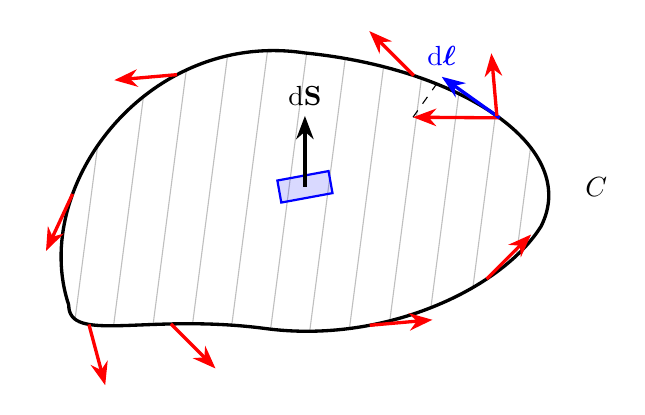
\begin{tikzpicture}[>=Stealth, thick]

  % Define the boundary path
  \def\boundary{
    (-3,-1) .. controls (-3.5,0.5) and (-2,2.5) .. (0,2.2)
    .. controls (2,2) and (3.5,1) .. (3,0)
    .. controls (2.5,-0.8) and (1,-1.5) .. (-0.5,-1.3)
    .. controls (-2,-1.1) and (-3,-1.5) .. (-3,-1)
  }

  % Hatching on surface (clipped)
  \begin{scope}
    \clip \boundary;
    \foreach \x in {-3.5,-3.0,...,3.5} {
      \draw[gray!50, thin] (\x,-1.8) -- (\x+0.6,2.8);
    }
  \end{scope}

  % Boundary curve C (black solid, no arrows), extract points along C
  \draw[very thick]
    (-3,-1)
    .. controls (-3.5,0.5) and (-2,2.5) ..
    coordinate[pos=0.3] (R1) coordinate[pos=0.7] (R2) (0,2.2)
    .. controls (2,2) and (3.5,1) ..
    coordinate[pos=0.25] (R3) coordinate[pos=0.5] (R4)
    coordinate[pos=0.51] (L) coordinate[pos=0.49] (L') (3,0)
    .. controls (2.5,-0.8) and (1,-1.5) ..
    coordinate[pos=0.3] (R5) coordinate[pos=0.7] (R6) (-0.5,-1.3)
    .. controls (-2,-1.1) and (-3,-1.5) ..
    coordinate[pos=0.3] (R7) coordinate[pos=0.7] (R8) (-3,-1);

  % Micro surface element at center
  \coordinate (P) at (0,0.5);
  \coordinate (dA) at (-0.3,-0.2);
  \coordinate (dB) at (0.35,-0.08);
  \fill[blue, opacity=0.15]
    ($(P)+(dA)$) -- ($(P)+(dB)$) -- ($(P)-(dA)$) -- ($(P)-(dB)$) -- cycle;
  \draw[blue, thick]
    ($(P)+(dA)$) -- ($(P)+(dB)$) -- ($(P)-(dA)$) -- ($(P)-(dB)$) -- cycle;

  % dS arrow from center of surface
  \draw[->, very thick] (P) -- ++(0,0.9) node[above] {$\mathrm{d}\mathbf{S}$};

  % Blue dℓ: tangent to C
  \pgfmathanglebetweenpoints{\pgfpointanchor{L}{center}}{\pgfpointanchor{L'}{center}}
  \edef\tangL{\pgfmathresult}
  % Red vector at L: its tangent projection = dℓ (length 0.9)
  \pgfmathsetmacro{\redang}{\tangL+35}
  \pgfmathsetmacro{\redlen}{0.9/cos(35)}
  \draw[->, red, very thick] (L) -- ++(\redang:\redlen);
  % Dashed projection
  \draw[dashed, thin] ([shift={(\redang:\redlen)}]L) -- ([shift={(\tangL:0.9)}]L);
  % Blue dℓ
  \draw[->, blue, very thick] (L) -- ++(\tangL:0.9)
    node[above] {$\mathrm{d}\boldsymbol{\ell}$};

  % Red vectors along C (roughly counterclockwise, but not exactly tangent)
  \draw[->, red, very thick] (R1) -- ++(245:0.8);
  \draw[->, red, very thick] (R2) -- ++(185:0.8);
  \draw[->, red, very thick] (R3) -- ++(135:0.8);
  \draw[->, red, very thick] (R4) -- ++(95:0.8);
  \draw[->, red, very thick] (R5) -- ++(45:0.8);
  \draw[->, red, very thick] (R6) -- ++(5:0.8);
  \draw[->, red, very thick] (R7) -- ++(315:0.8);
  \draw[->, red, very thick] (R8) -- ++(285:0.8);

  % C label
  \node at (3.7,0.5) {$C$};

\end{tikzpicture}
\end{document}
